\chapter{Results and Analysis}
\label{ch:resultsAndAnalysis}


% \engExpl{Sometimes this is split into two chapters.\\Keep in mind: How you are going to evaluate what you have done? What are your metrics?\\Analysis of your data and proposed solution\\Does this meet the goals which you had when you started?}


This chapter will present and analyse the results of the research conducted in this thesis.


% \sweExpl{I detta kapitel presenterar vi resultaten och diskutera dem.\\Ibland delas detta upp i två kapitel.\\Hur du ska utvärdera vad du har gjort? Vad är din statistik?\\Analys av data och föreslagen lösning\\Innebär detta att uppfyllelse av de mål som du hade när du började?}


% \sweExpl{Huvudsakliga resultat}


\section{Feasibility of building an AI assistant on open source technologies}


One of the goals of the research in this thesis was, as outlined in section~\ref{sec:goals}, to assess the feasibility of building an AI-assistant on open-source technologies and deploying the agent in an academic setting. This section will outline the results and showcase the impact open source tooling had on the implementation of the AI assistant.


\subsection{How popular was the system}


The system was developed during the spring of 2024 and gradually deployed to seven real courses at KTH starting on the 18th of April 2024. The students in the courses that participated in the study held a total of 656chats and sent 2373messages. As can be seen in \autoref{fig:usage_01_cumulative_number_of_chats} and \autoref{fig:usage_08_number_of_messages_per_day} these steadily increased over the course of the study as students initiated new chats with the assistant.


\begin{figure}[H]
    \centering
    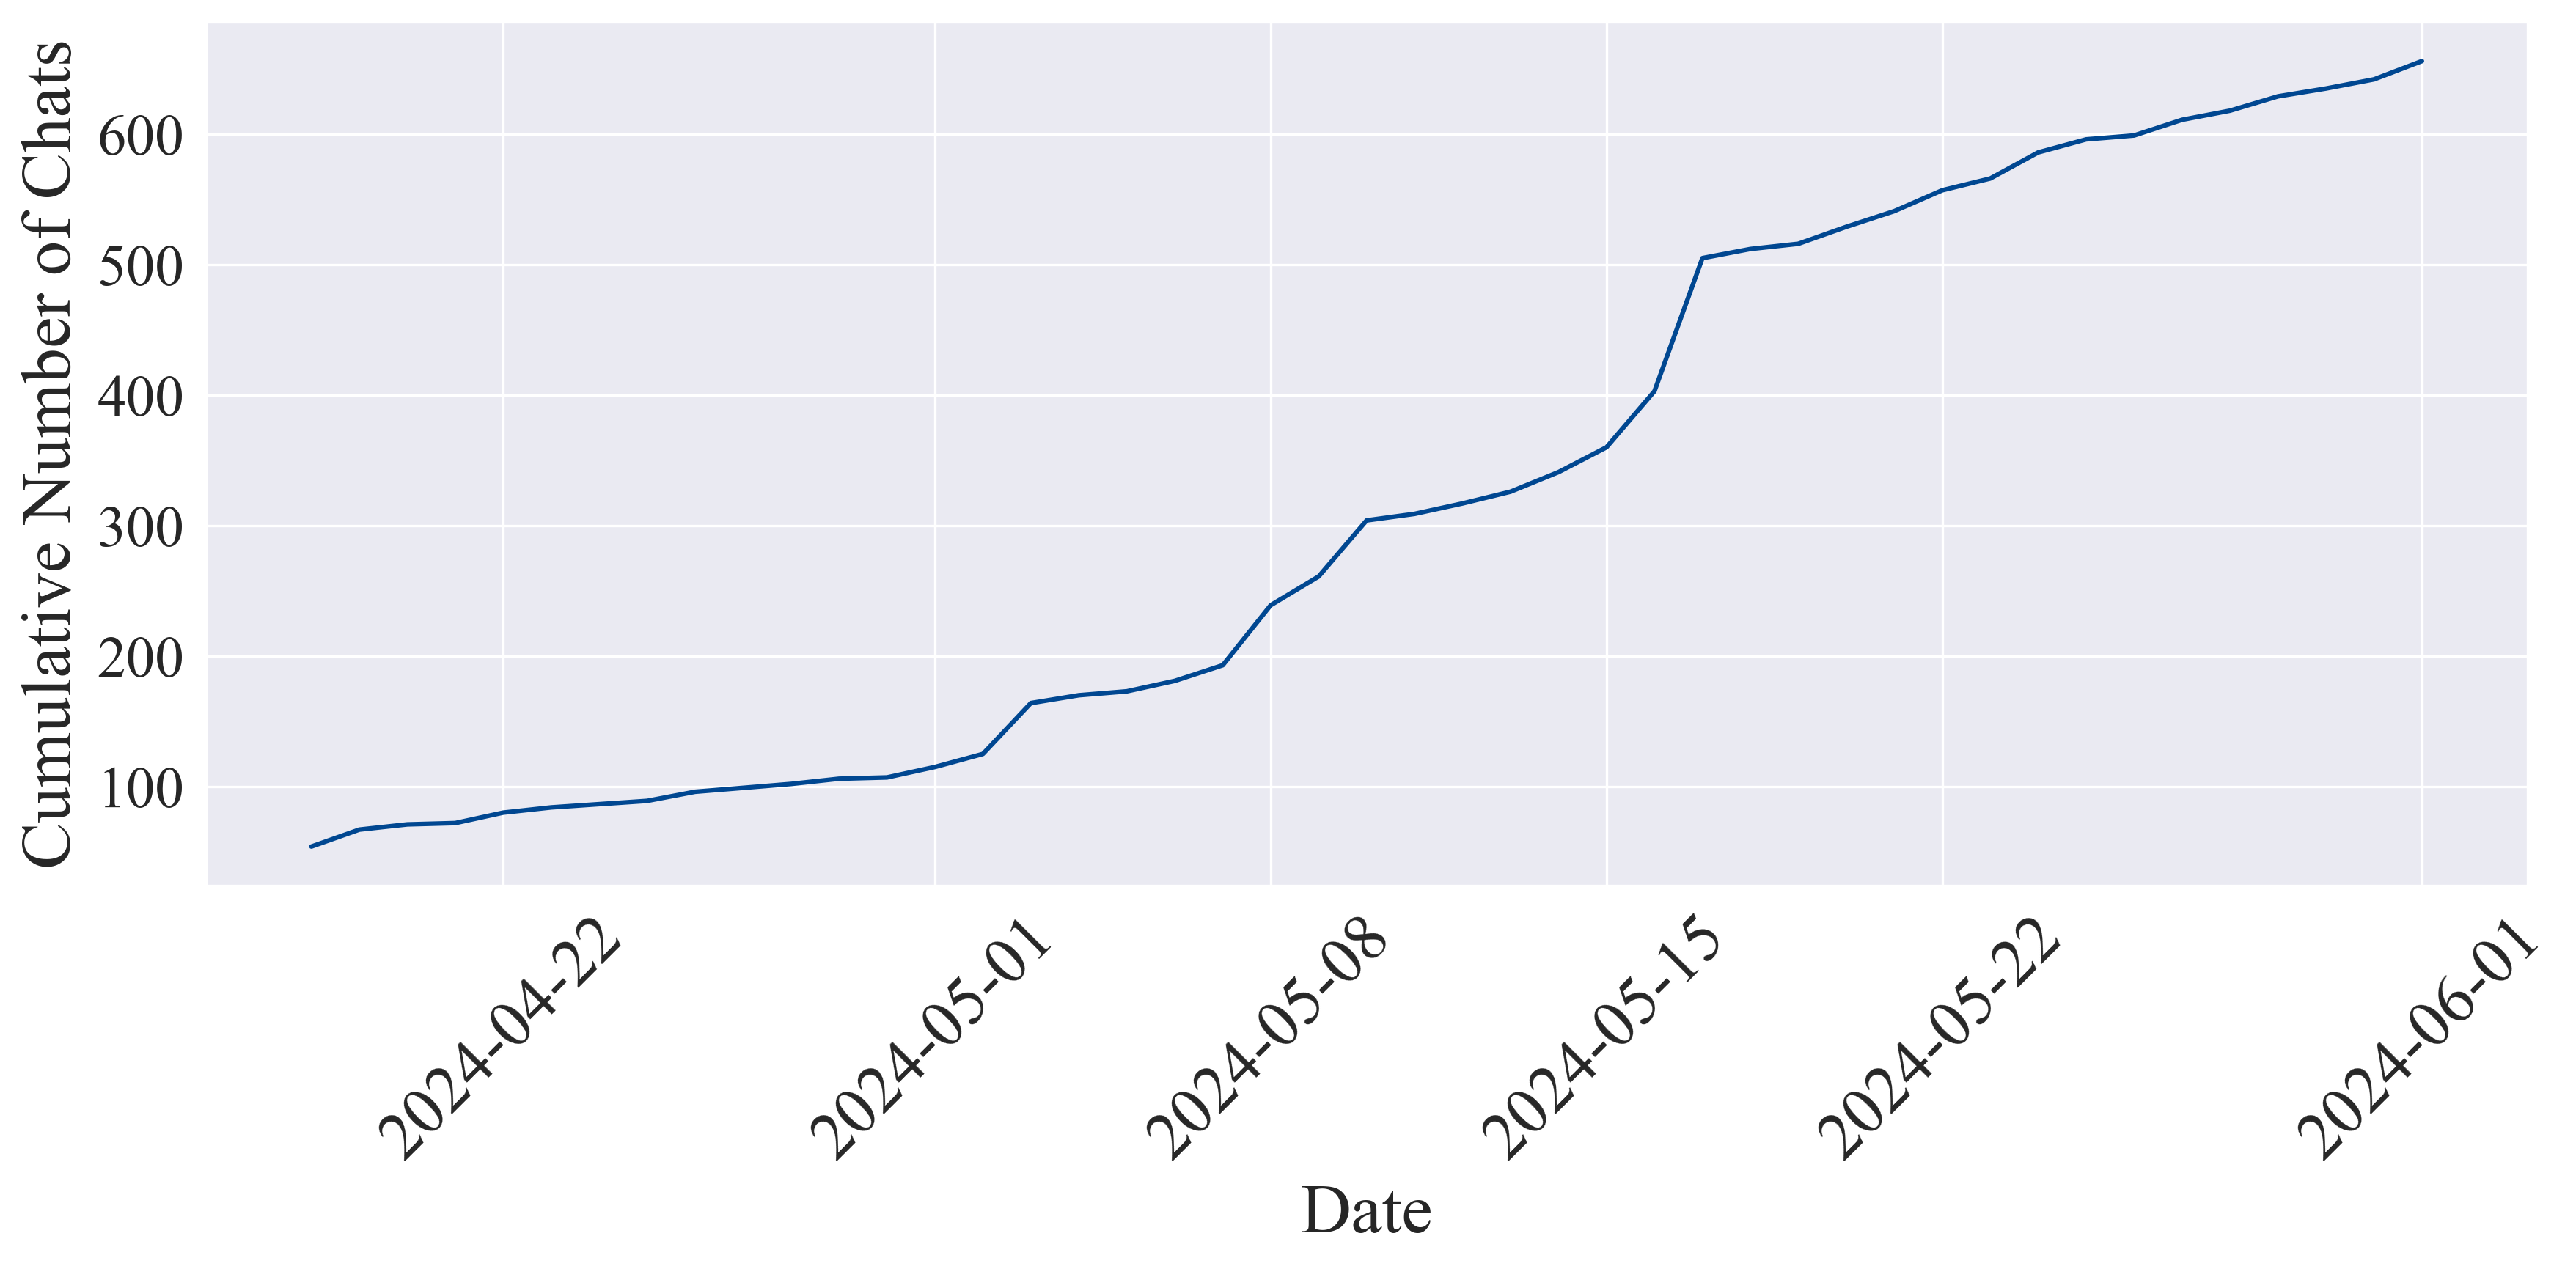
\includegraphics[width=1\textwidth]{results/plots/assets/usage-01-cumulative-number-of-chats.png}
    \caption{Cumulative number of chats started by users participating in the study}
    \label{fig:usage_01_cumulative_number_of_chats}
\end{figure}


\begin{figure}[H]
    \centering
    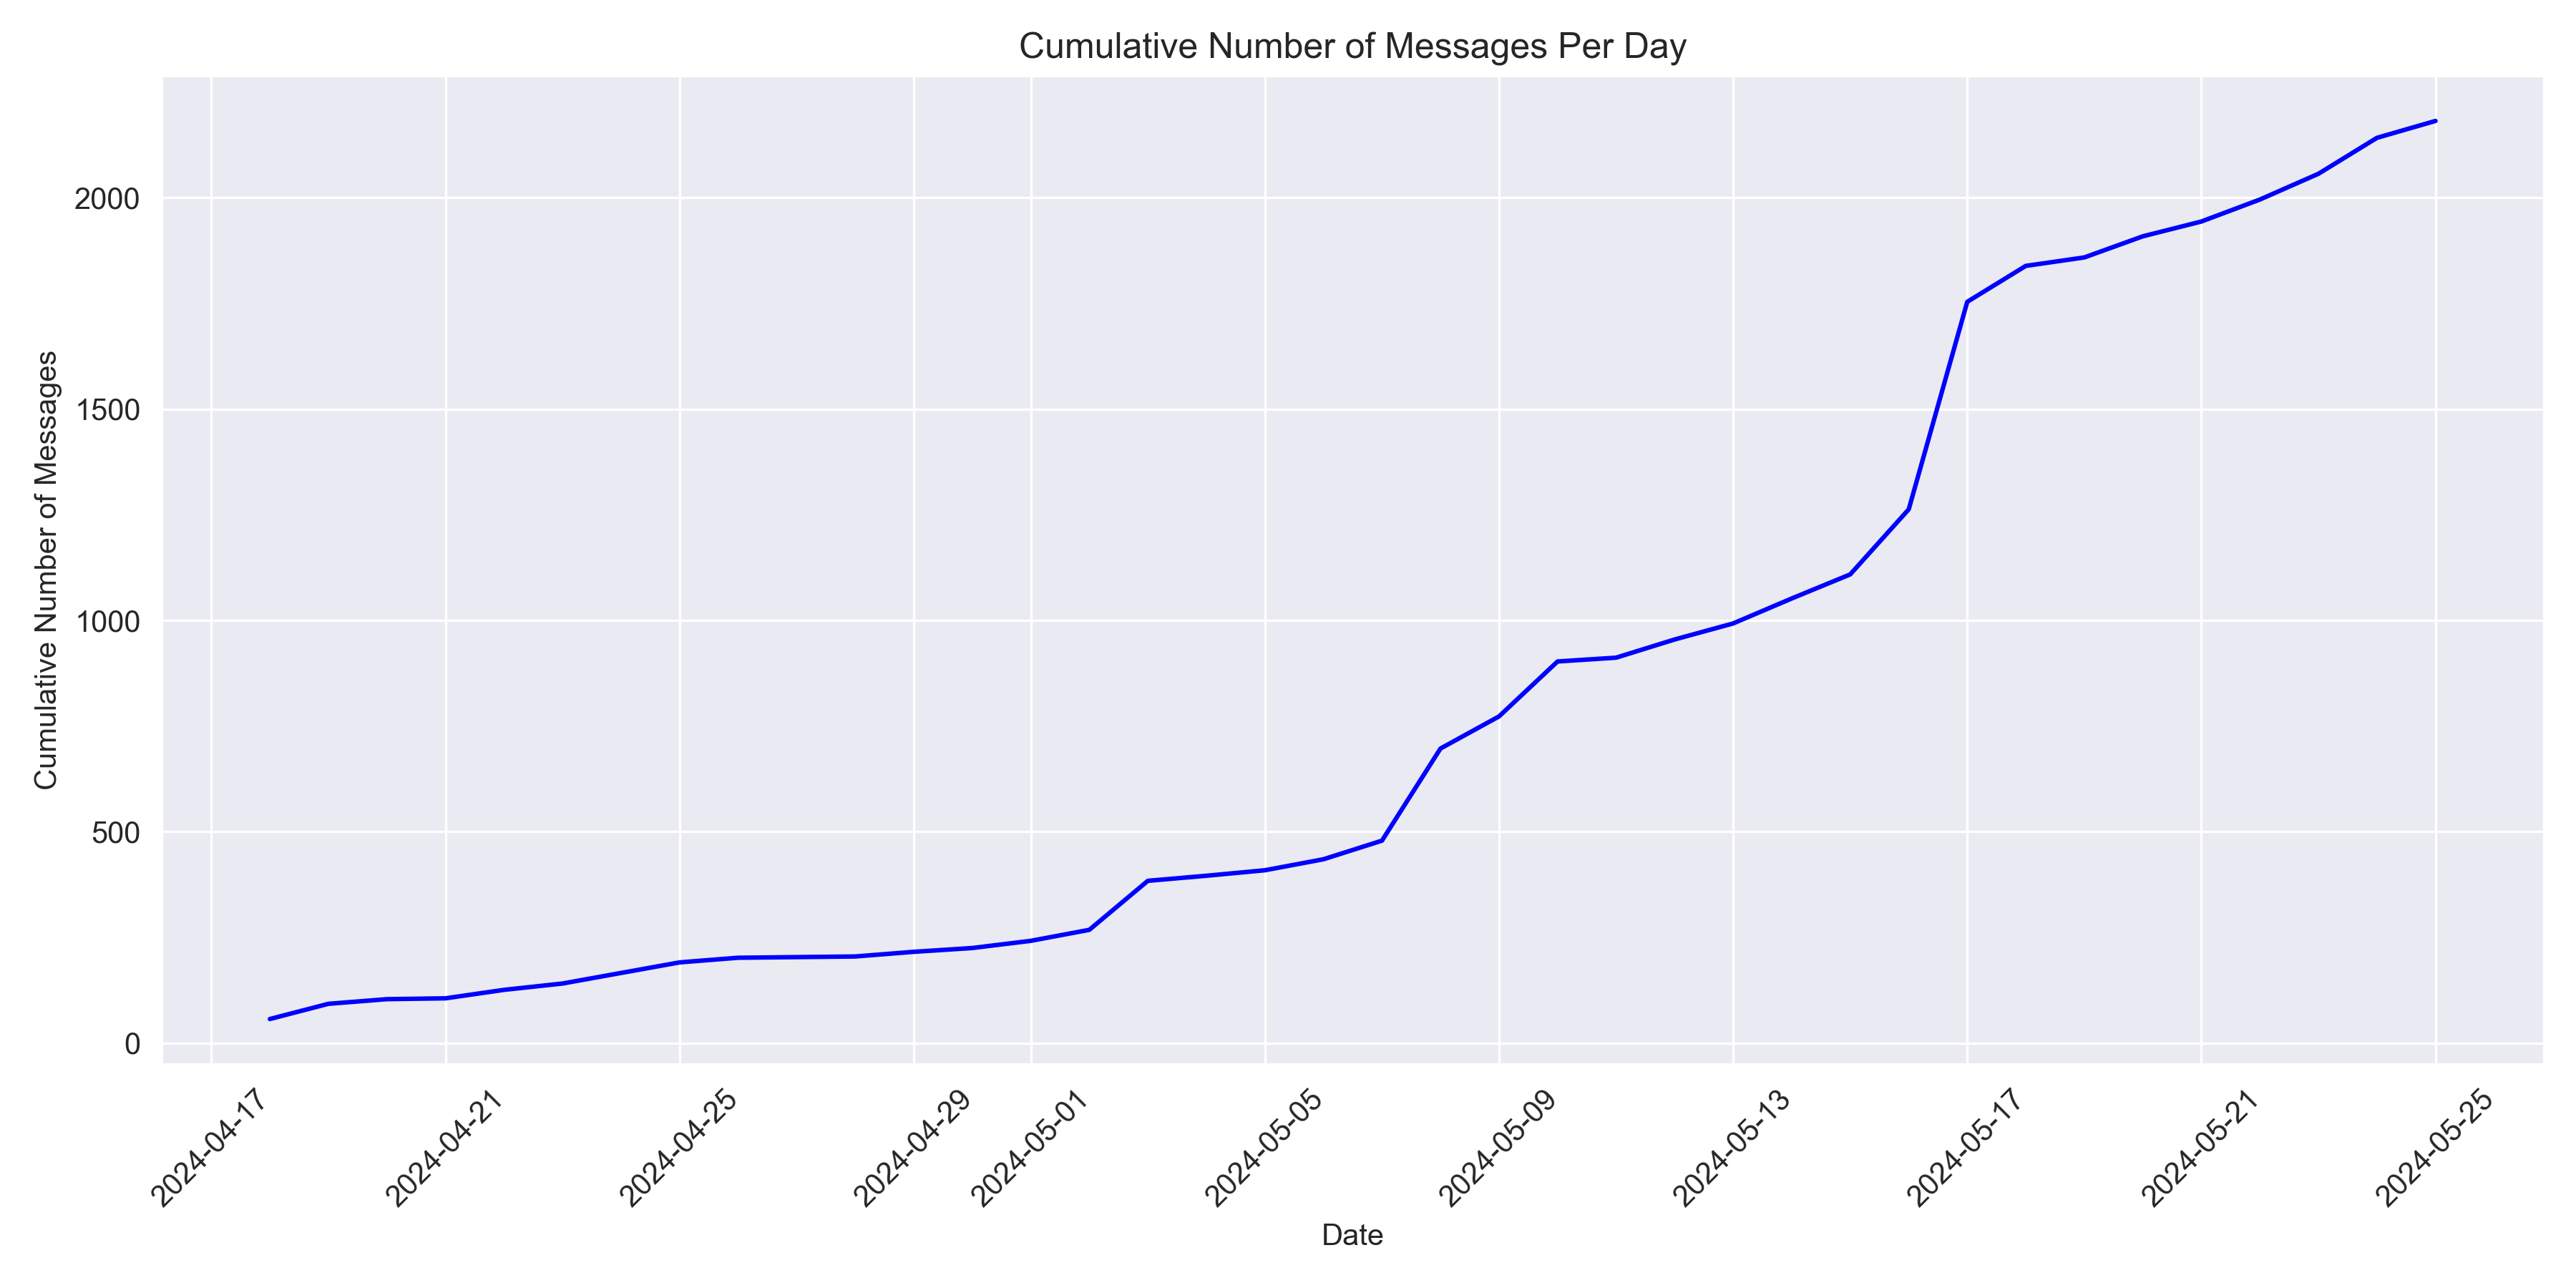
\includegraphics[width=1\textwidth]{results/plots/assets/usage-08-number-of-messages-per-day.png}
    \caption{Cumulative number of messages per day}
    \label{fig:usage_08_number_of_messages_per_day}
\end{figure}


Separating the chats initiated in the separate course rooms we observe that some courses followed a fairly linear increase in the number of chats. One example of this is the course \textit{MG2040 Assembly Technology 6.0 credits}, which can be seen in figure~\ref{fig:usage_02_cumulative_number_of_chats_per_course}.


\begin{figure}[H]
    \centering
    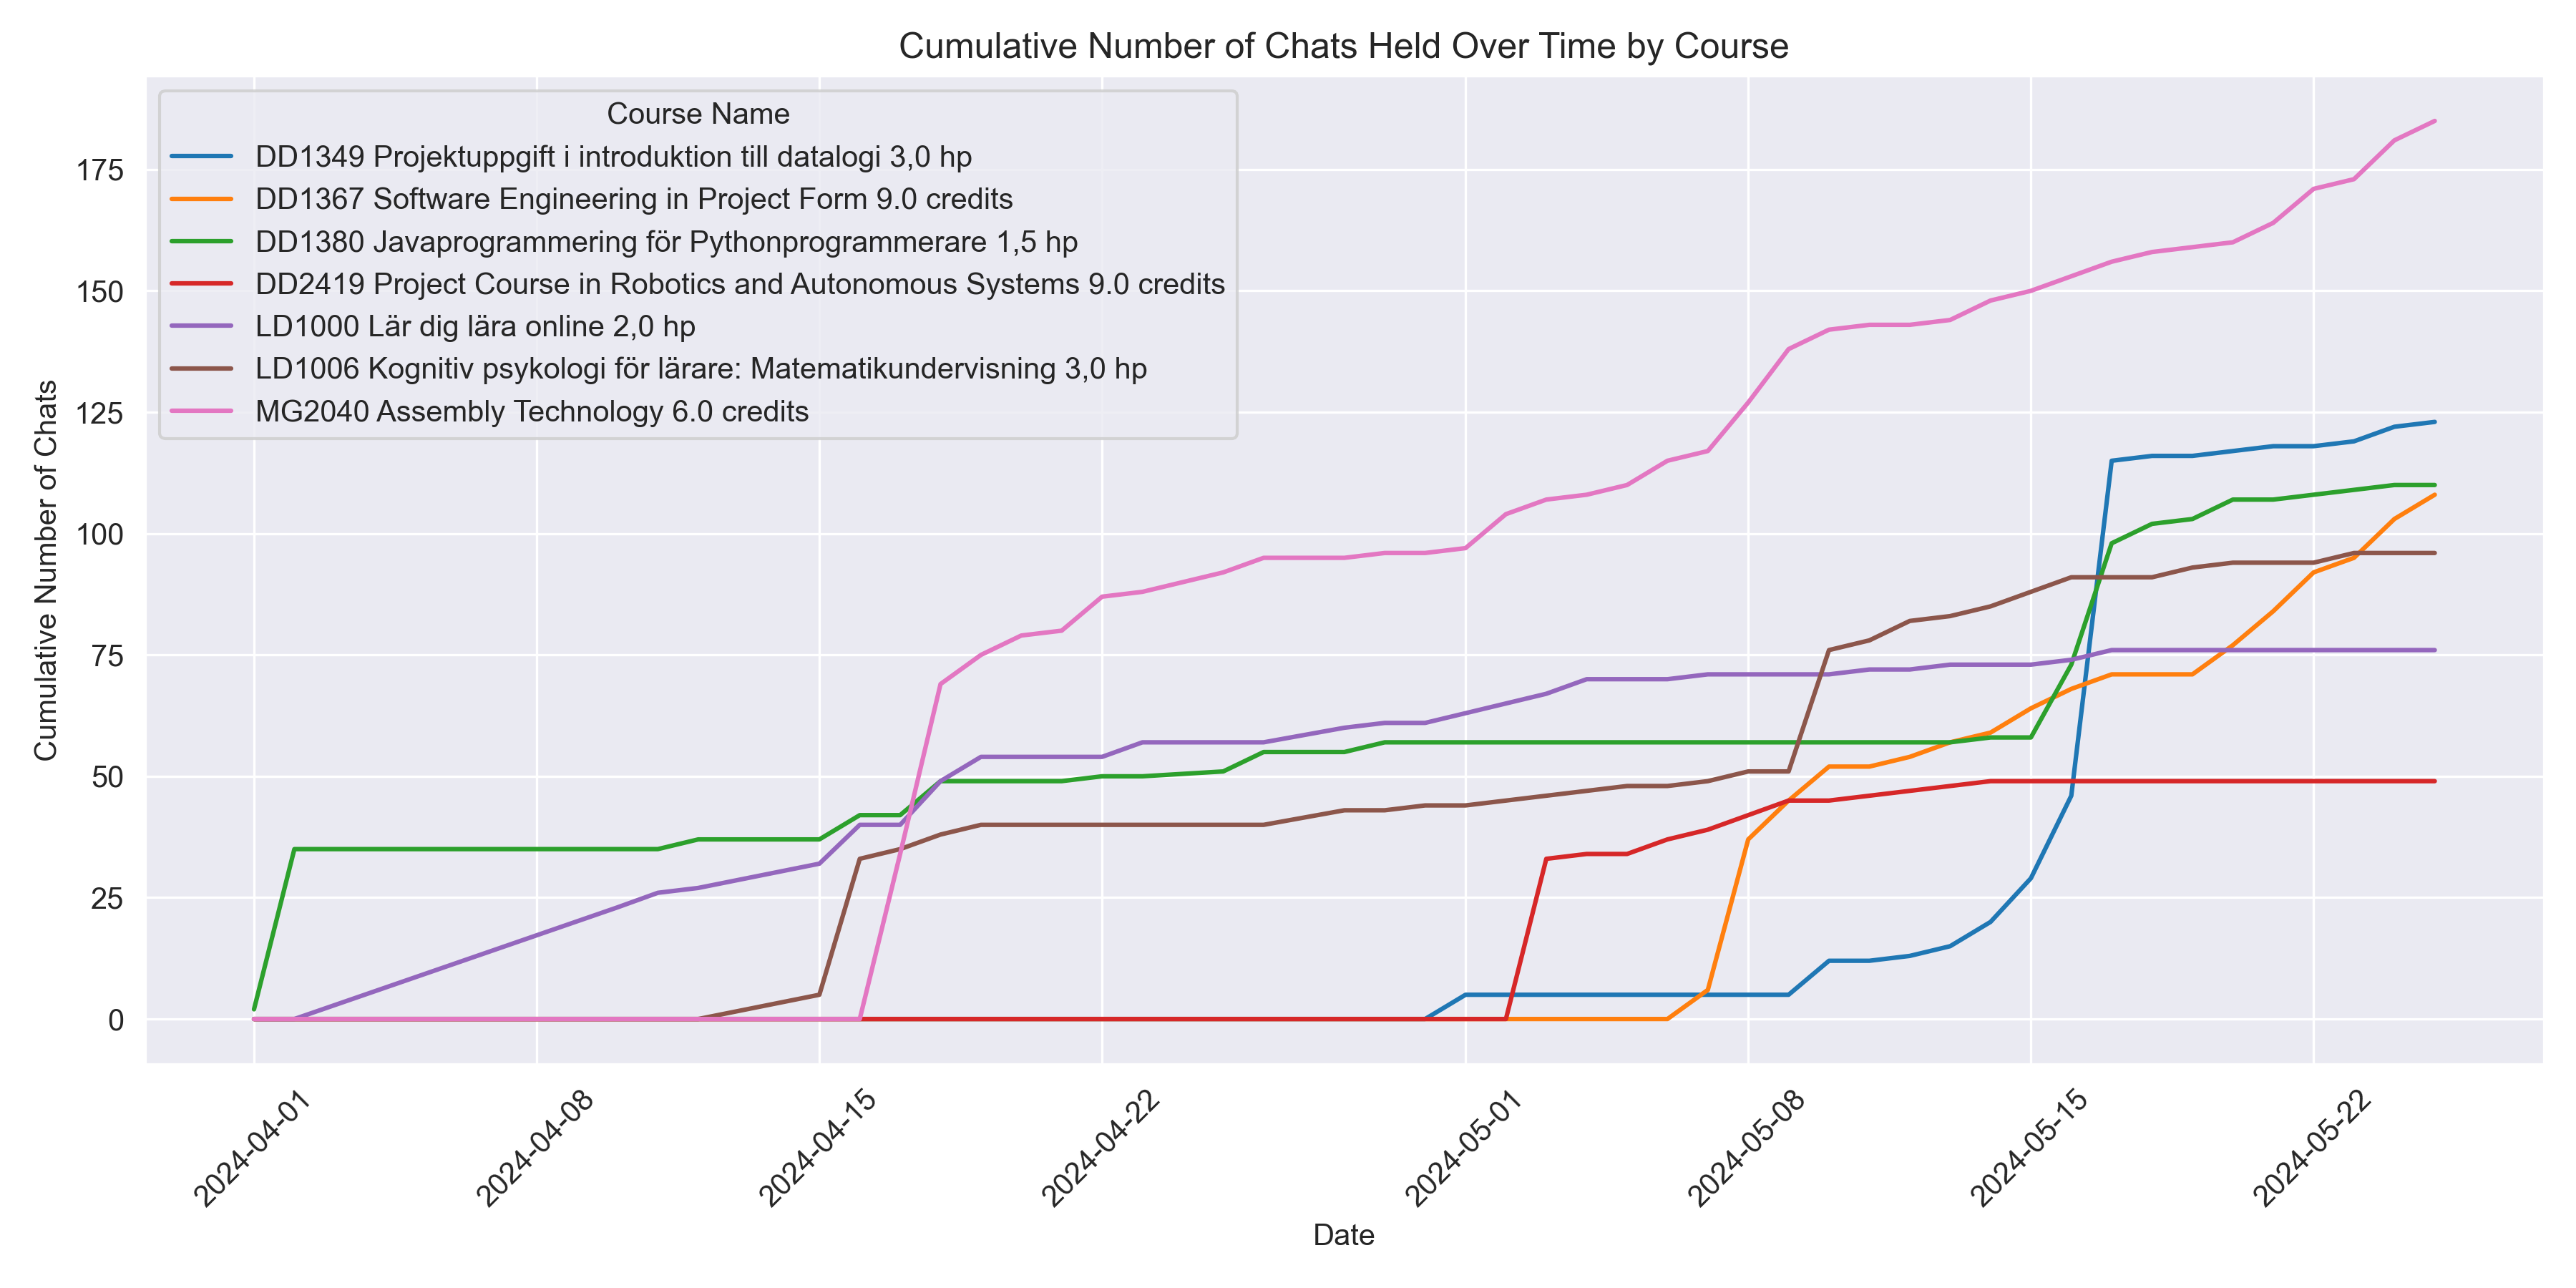
\includegraphics[width=\textwidth]{results/plots/assets/usage-02-cumulative-number-of-chats-per-course.png}
    \caption{Cumulative number of chats started by users participating in the study in each course}
    \label{fig:usage_02_cumulative_number_of_chats_per_course}
\end{figure}


Looking at other courses in figure~\ref{fig:usage_02_cumulative_number_of_chats_per_course} it is evident that not all courses follow the same pattern as \textit{MG2040}. Some courses initially have very few chats due to the chatbot not being deployed simultaneously across all courses. \autoref{tab:course_start_dates} details the start dates for each course. For instance, \textit{DD1349 Projektuppgift i introduktion till datalogi 3,0 hp} exhibits a steep increase in users when it launched, followed by no further growth. This is because the course officially ended shortly after the chatbot was introduced. In all courses participating in the study, the chatbot was deployed well after the courses had already begun, therefore a similar pattern can be seen in many other courses.


\begin{table}[H]
\centering
{\scriptsize
\begin{tabularx}{\textwidth}{@{}X c@{}}
\toprule
\textbf{Course} & \textbf{Go live date} \\ \midrule
LD1000 Lär dig lära online 2,0 hp & 2024-04-17 \\
LD1006 Kognitiv psykologi för lärare: Matematikundervisning 3,0 hp & 2024-04-17 \\
MG2040 Assembly Technology 6.0 credits & 2024-04-17 \\
DD1349 Projektuppgift i introduktion till datalogi 3,0 hp & 2024-05-01 \\
DD2419 Project Course in Robotics and Autonomous Systems 9.0 credits & 2024-05-03 \\
DD1367 Software Engineering in Project Form 9.0 credits & 2024-05-07 \\
DD1380 Javaprogrammering för Pythonprogrammerare 1,5 hp & 2024-05-13 \\
\bottomrule
\end{tabularx}
}
\vspace{2mm}
\caption{The start dates for each course, when the bot was deployed in each canvas course room.}
\label{tab:course_start_dates}
\end{table}



\autoref{fig:usage_03_number_of_chats_per_course} shows the total number of chats held in each course. The course \textit{MG2040} held the most, 151chats. \textit{DD1349} held the second most and \textit{DD1367} the third most, 123and 122chats respectively.


\begin{figure}[H]
    \centering
    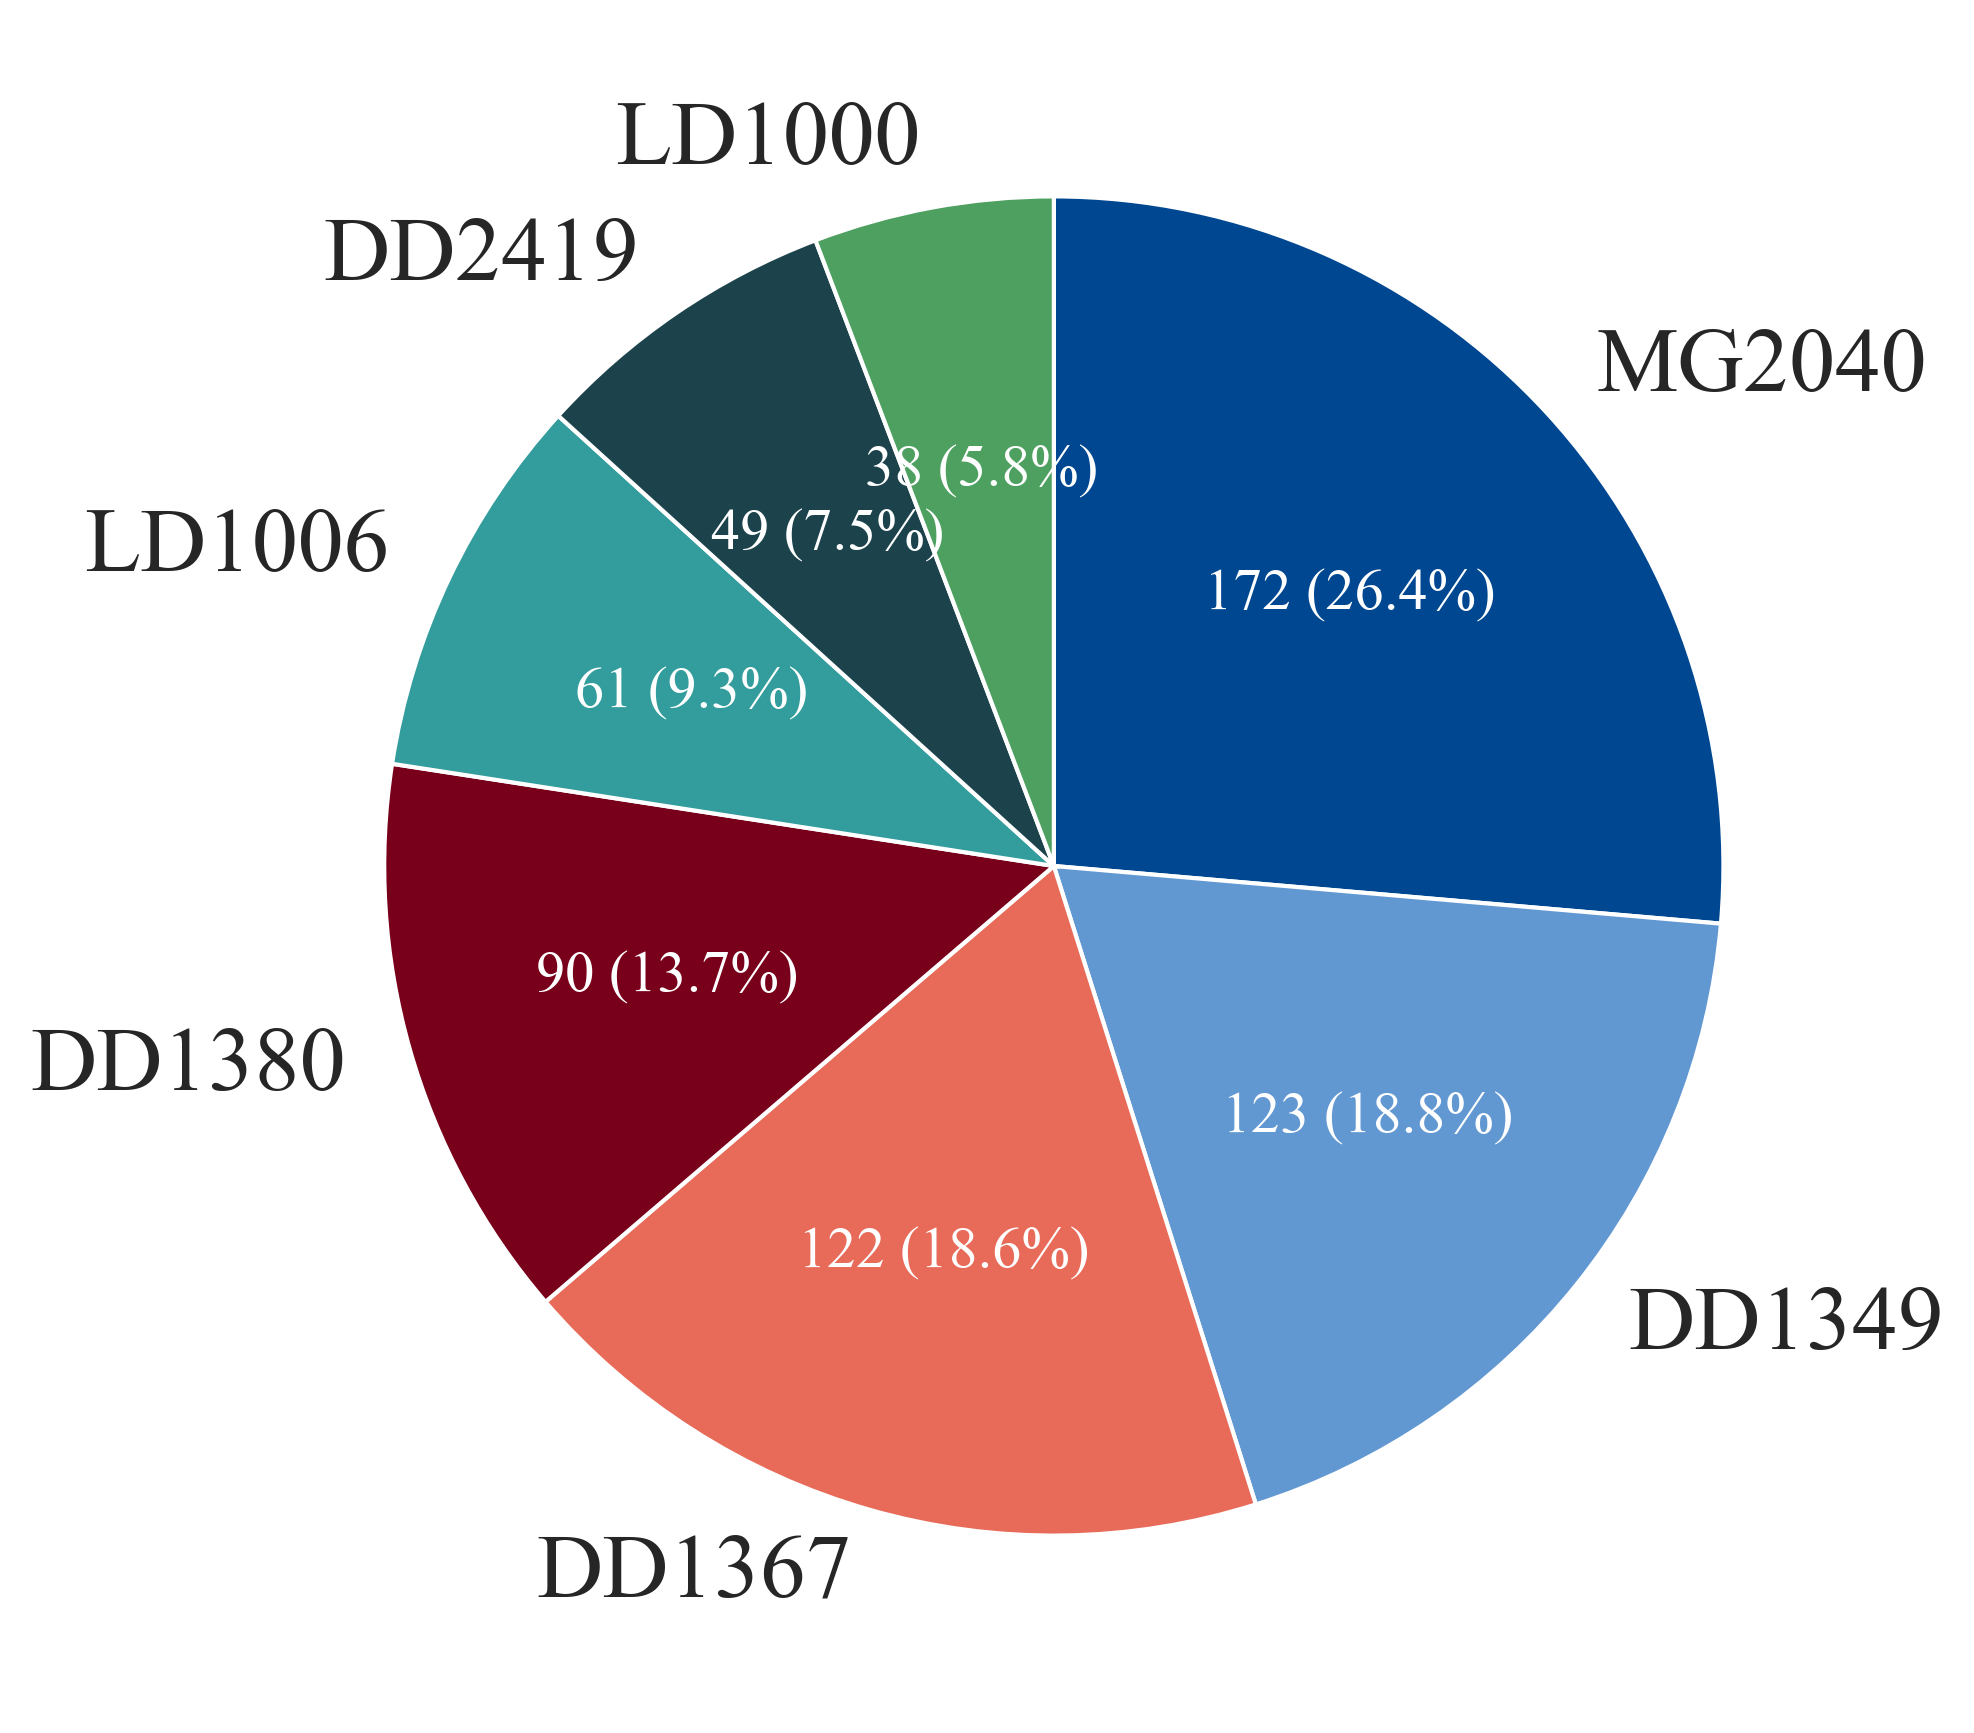
\includegraphics[width=\textwidth]{results/plots/assets/usage-05-number-of-chats-per-course.png}
    \caption{Number of chats held by in each course}
    \label{fig:usage_03_number_of_chats_per_course}
\end{figure}




Looking at the number of sessions created in \autoref{fig:usage_06_number_of_sessions_per_day} and \autoref{fig:usage_07_number_of_sessions_per_day_and_course}, we can see a similar pattern linear pattern. A session is started whenever a user loads the application without already having loaded it before. A session is not tracked between devices, therefore a user would have two sessions if the same user accessed the chat on two different devices, such as a desktop and a mobile phone. However, the same session is used across courses.


\begin{figure}[H]
    \centering
    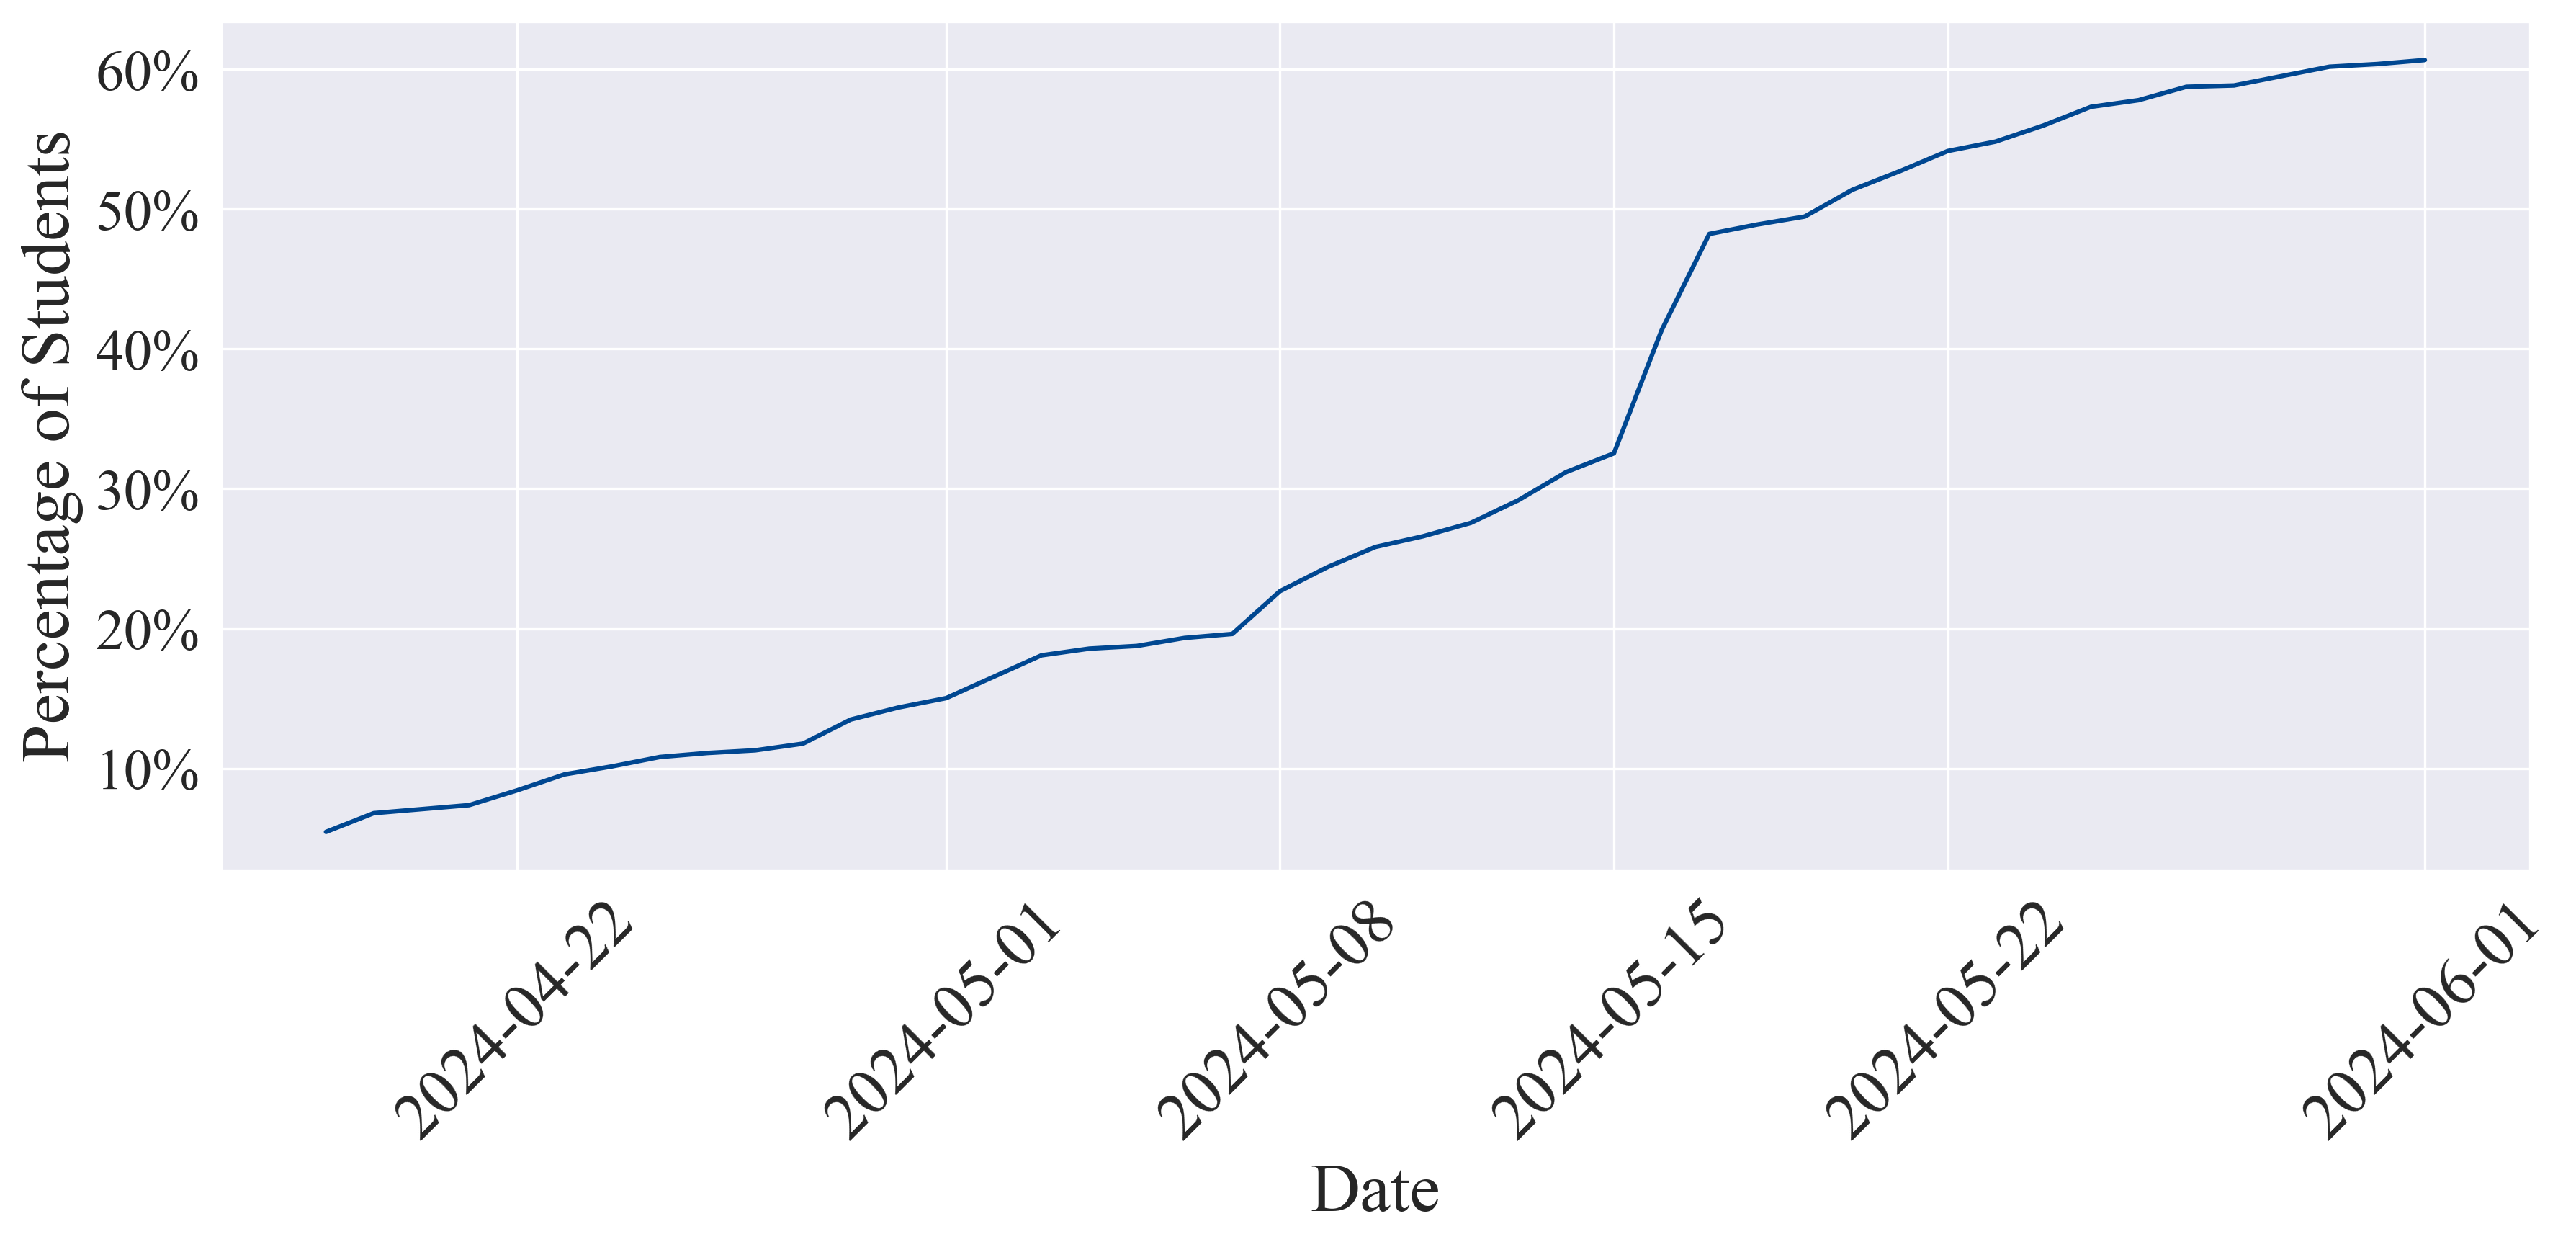
\includegraphics[width=\textwidth]{results/plots/assets/usage-06-number-of-sessions-per-day.png}
    \caption{Cumulative number of users as percentage of number of users in all participating courses that had started a chat}
    \label{fig:usage_06_number_of_sessions_per_day}
\end{figure}


\begin{figure}[H]
    \centering
    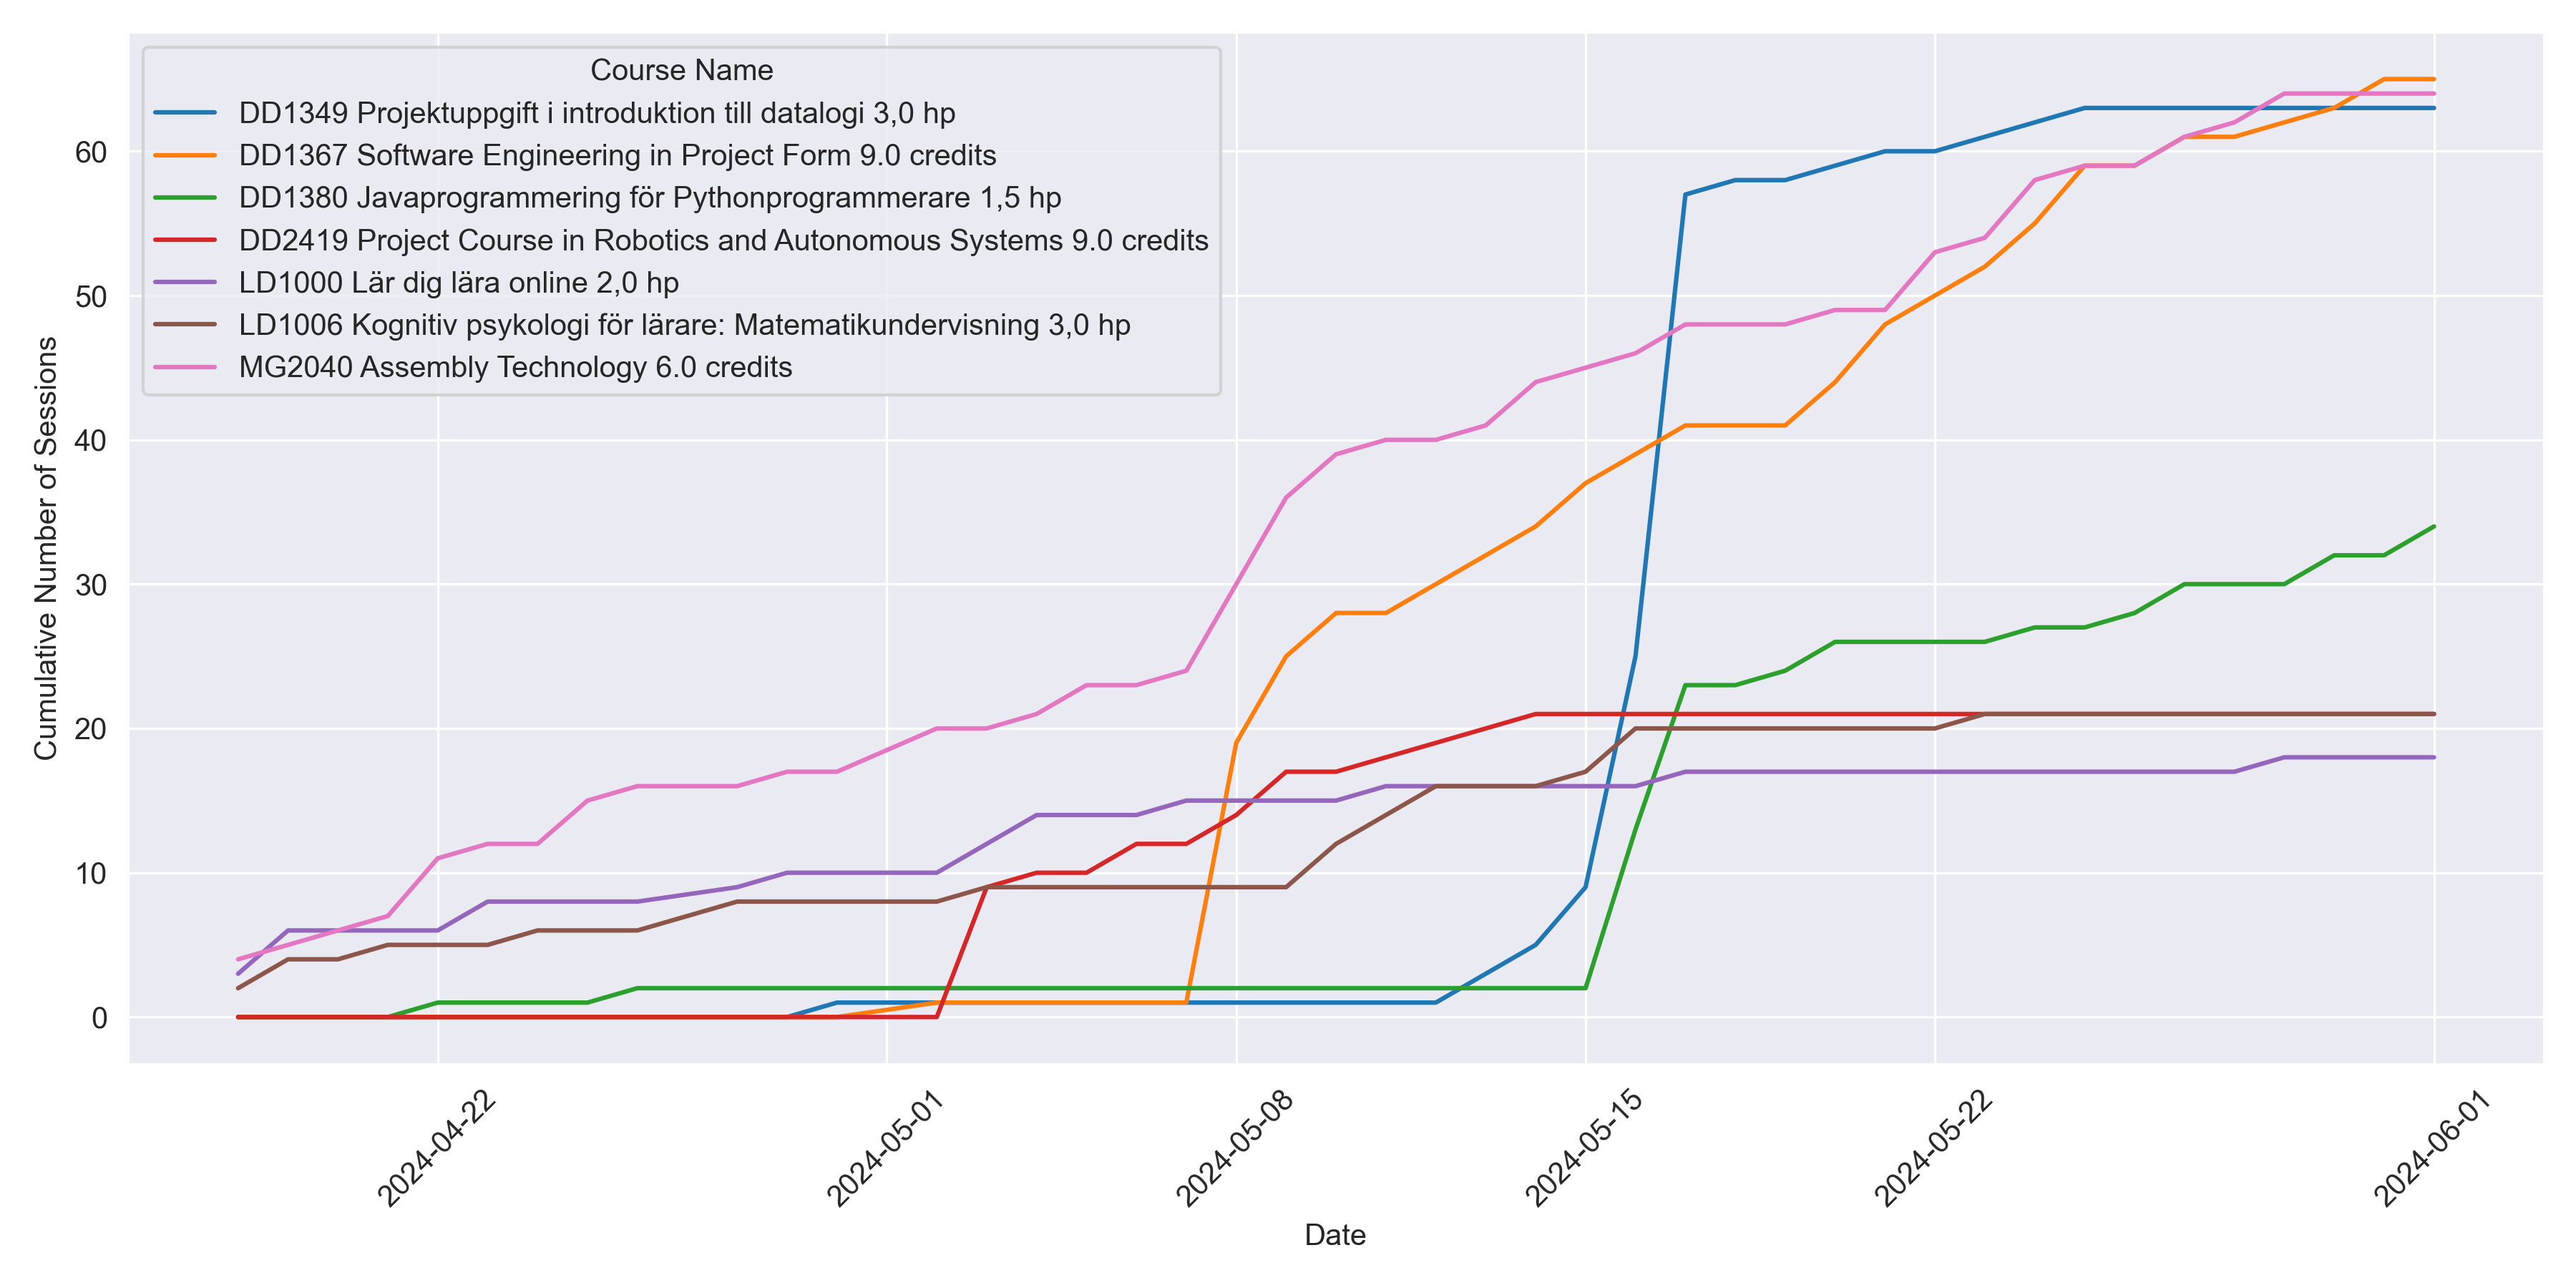
\includegraphics[width=1\textwidth]{results/plots/assets/usage-07-number-of-sessions-per-day-and-course.png}
    \caption{Cumulative number of users per day in each course, as a percentage of the course's students, that had started a chat}
    \label{fig:usage_07_number_of_sessions_per_day_and_course}
\end{figure}


Looking at the distribution of how many chats and messages is sent per session, as seen in figure \autoref{fig:usage_12_number_of_sessions_with_number_of_chats} and \autoref{fig:usage_13_number_of_sessions_with_number_of_messages} we can see that it was very common for users to only start one or two chats. Most users sent quite a few messages though. The average user held 2.22chats and sent 9.57messages.


\begin{figure}[H]
    \centering
    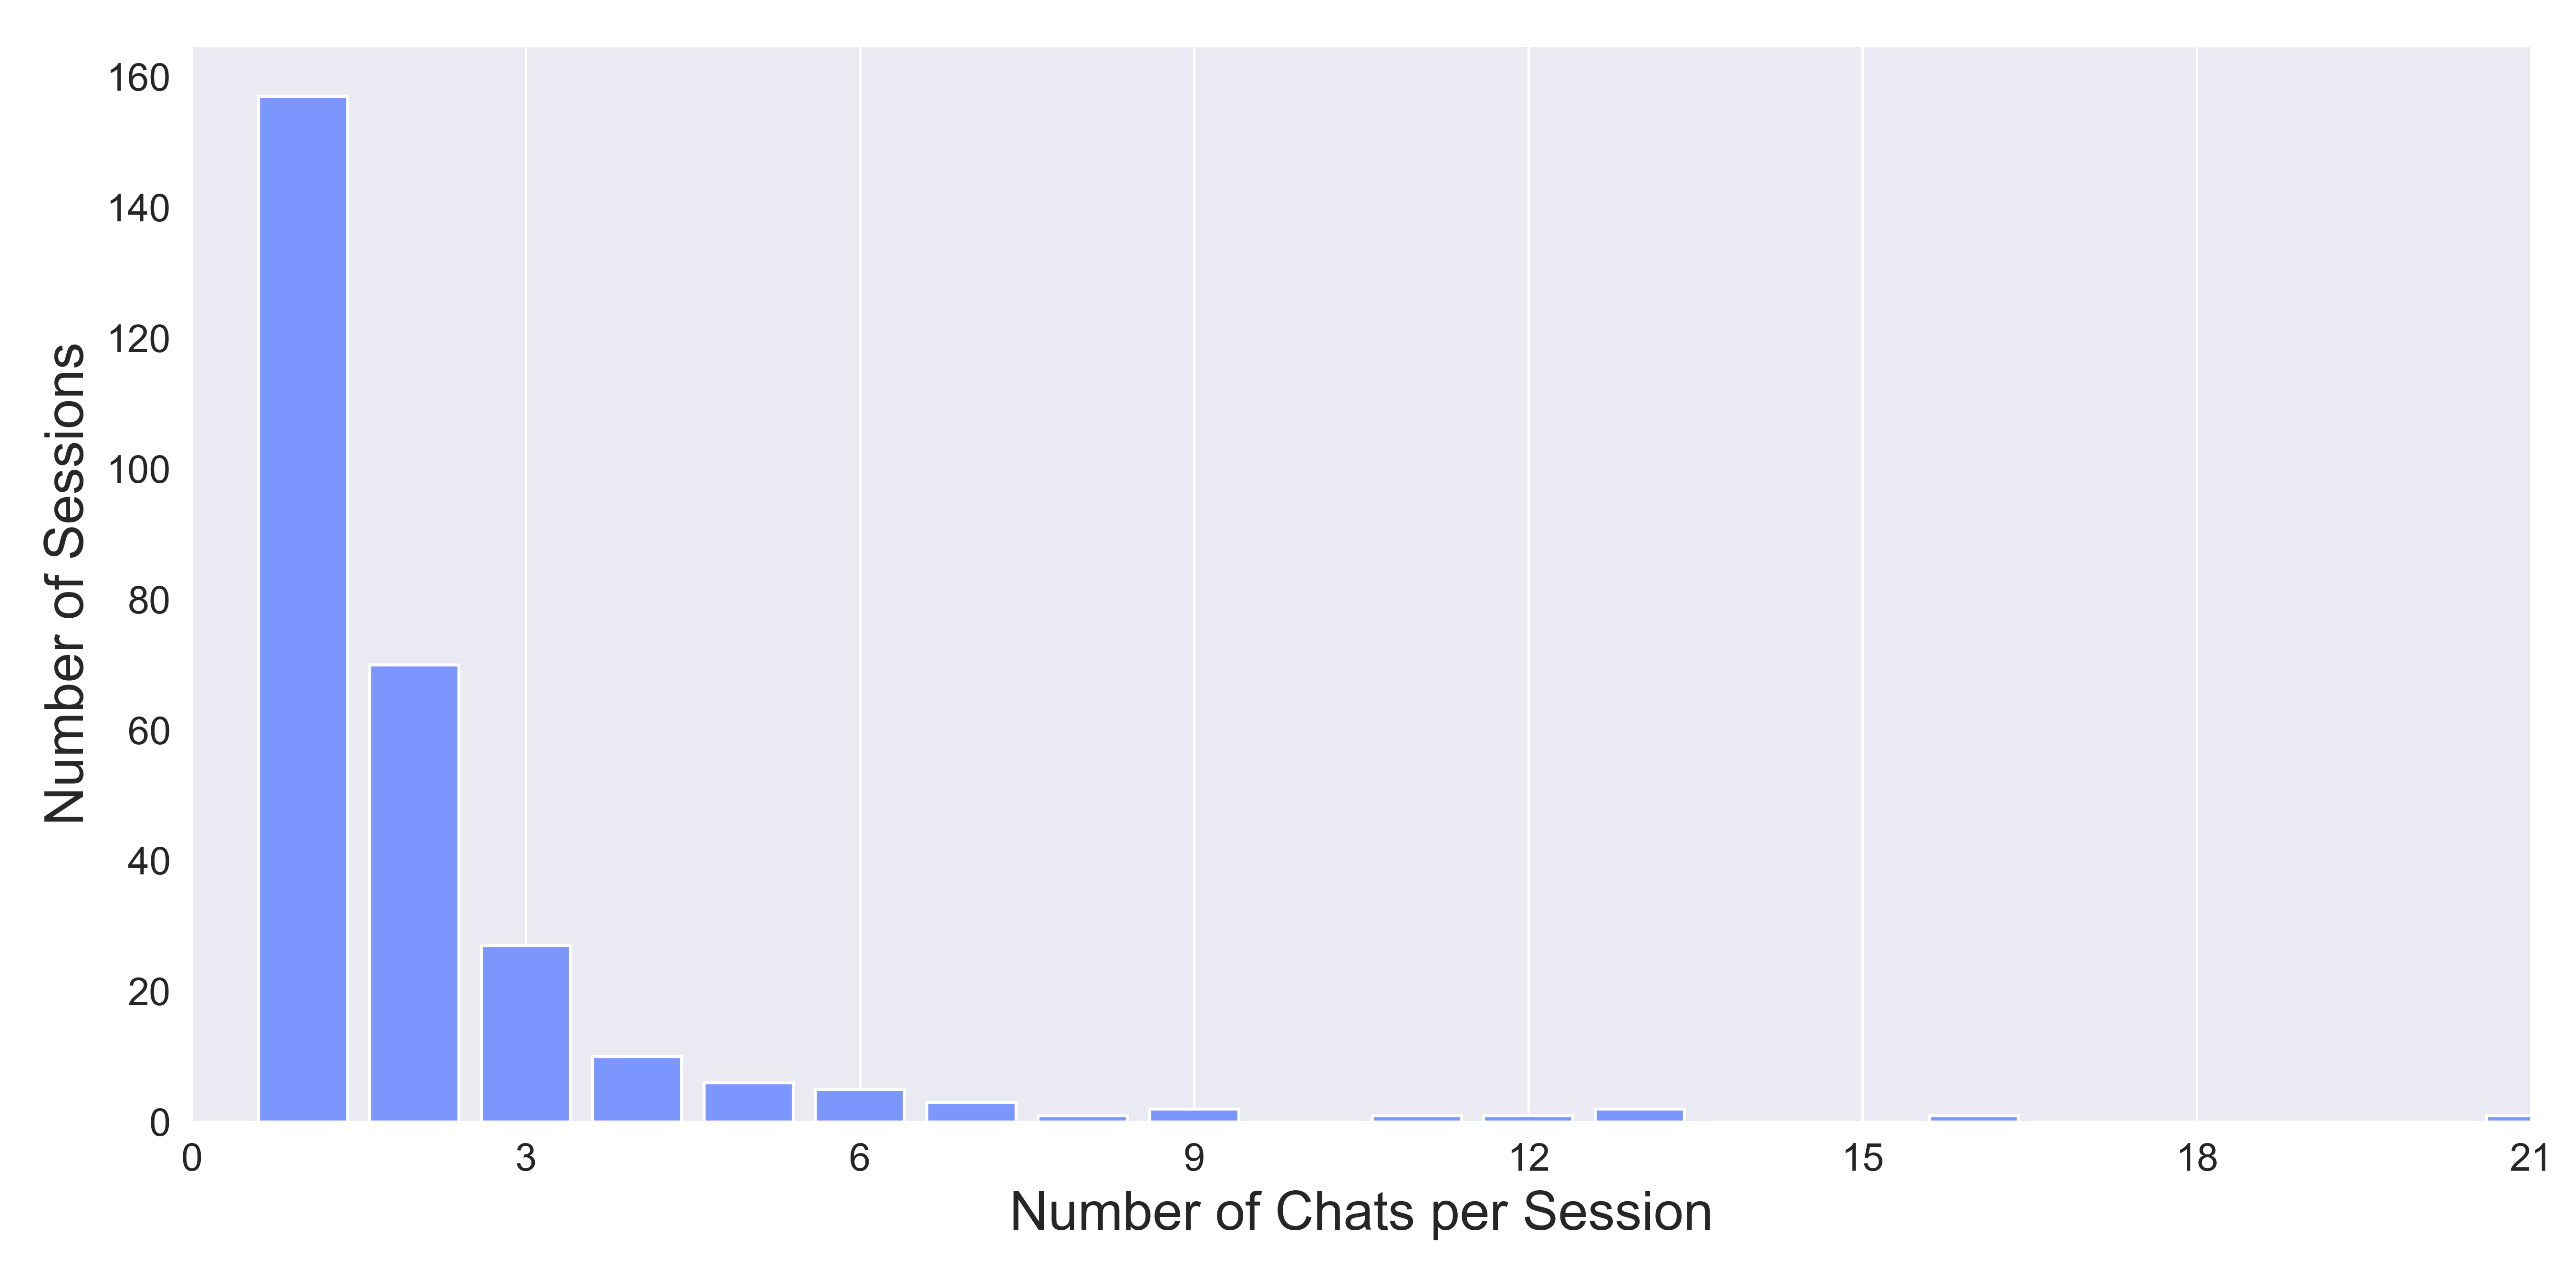
\includegraphics[width=\textwidth]{results/plots/assets/usage-12-number-of-sessions-with-number-of-chats.png}
    \caption{Number of sessions with each number of chats}
    \label{fig:usage_12_number_of_sessions_with_number_of_chats}
\end{figure}


\begin{figure}[H]
    \centering
    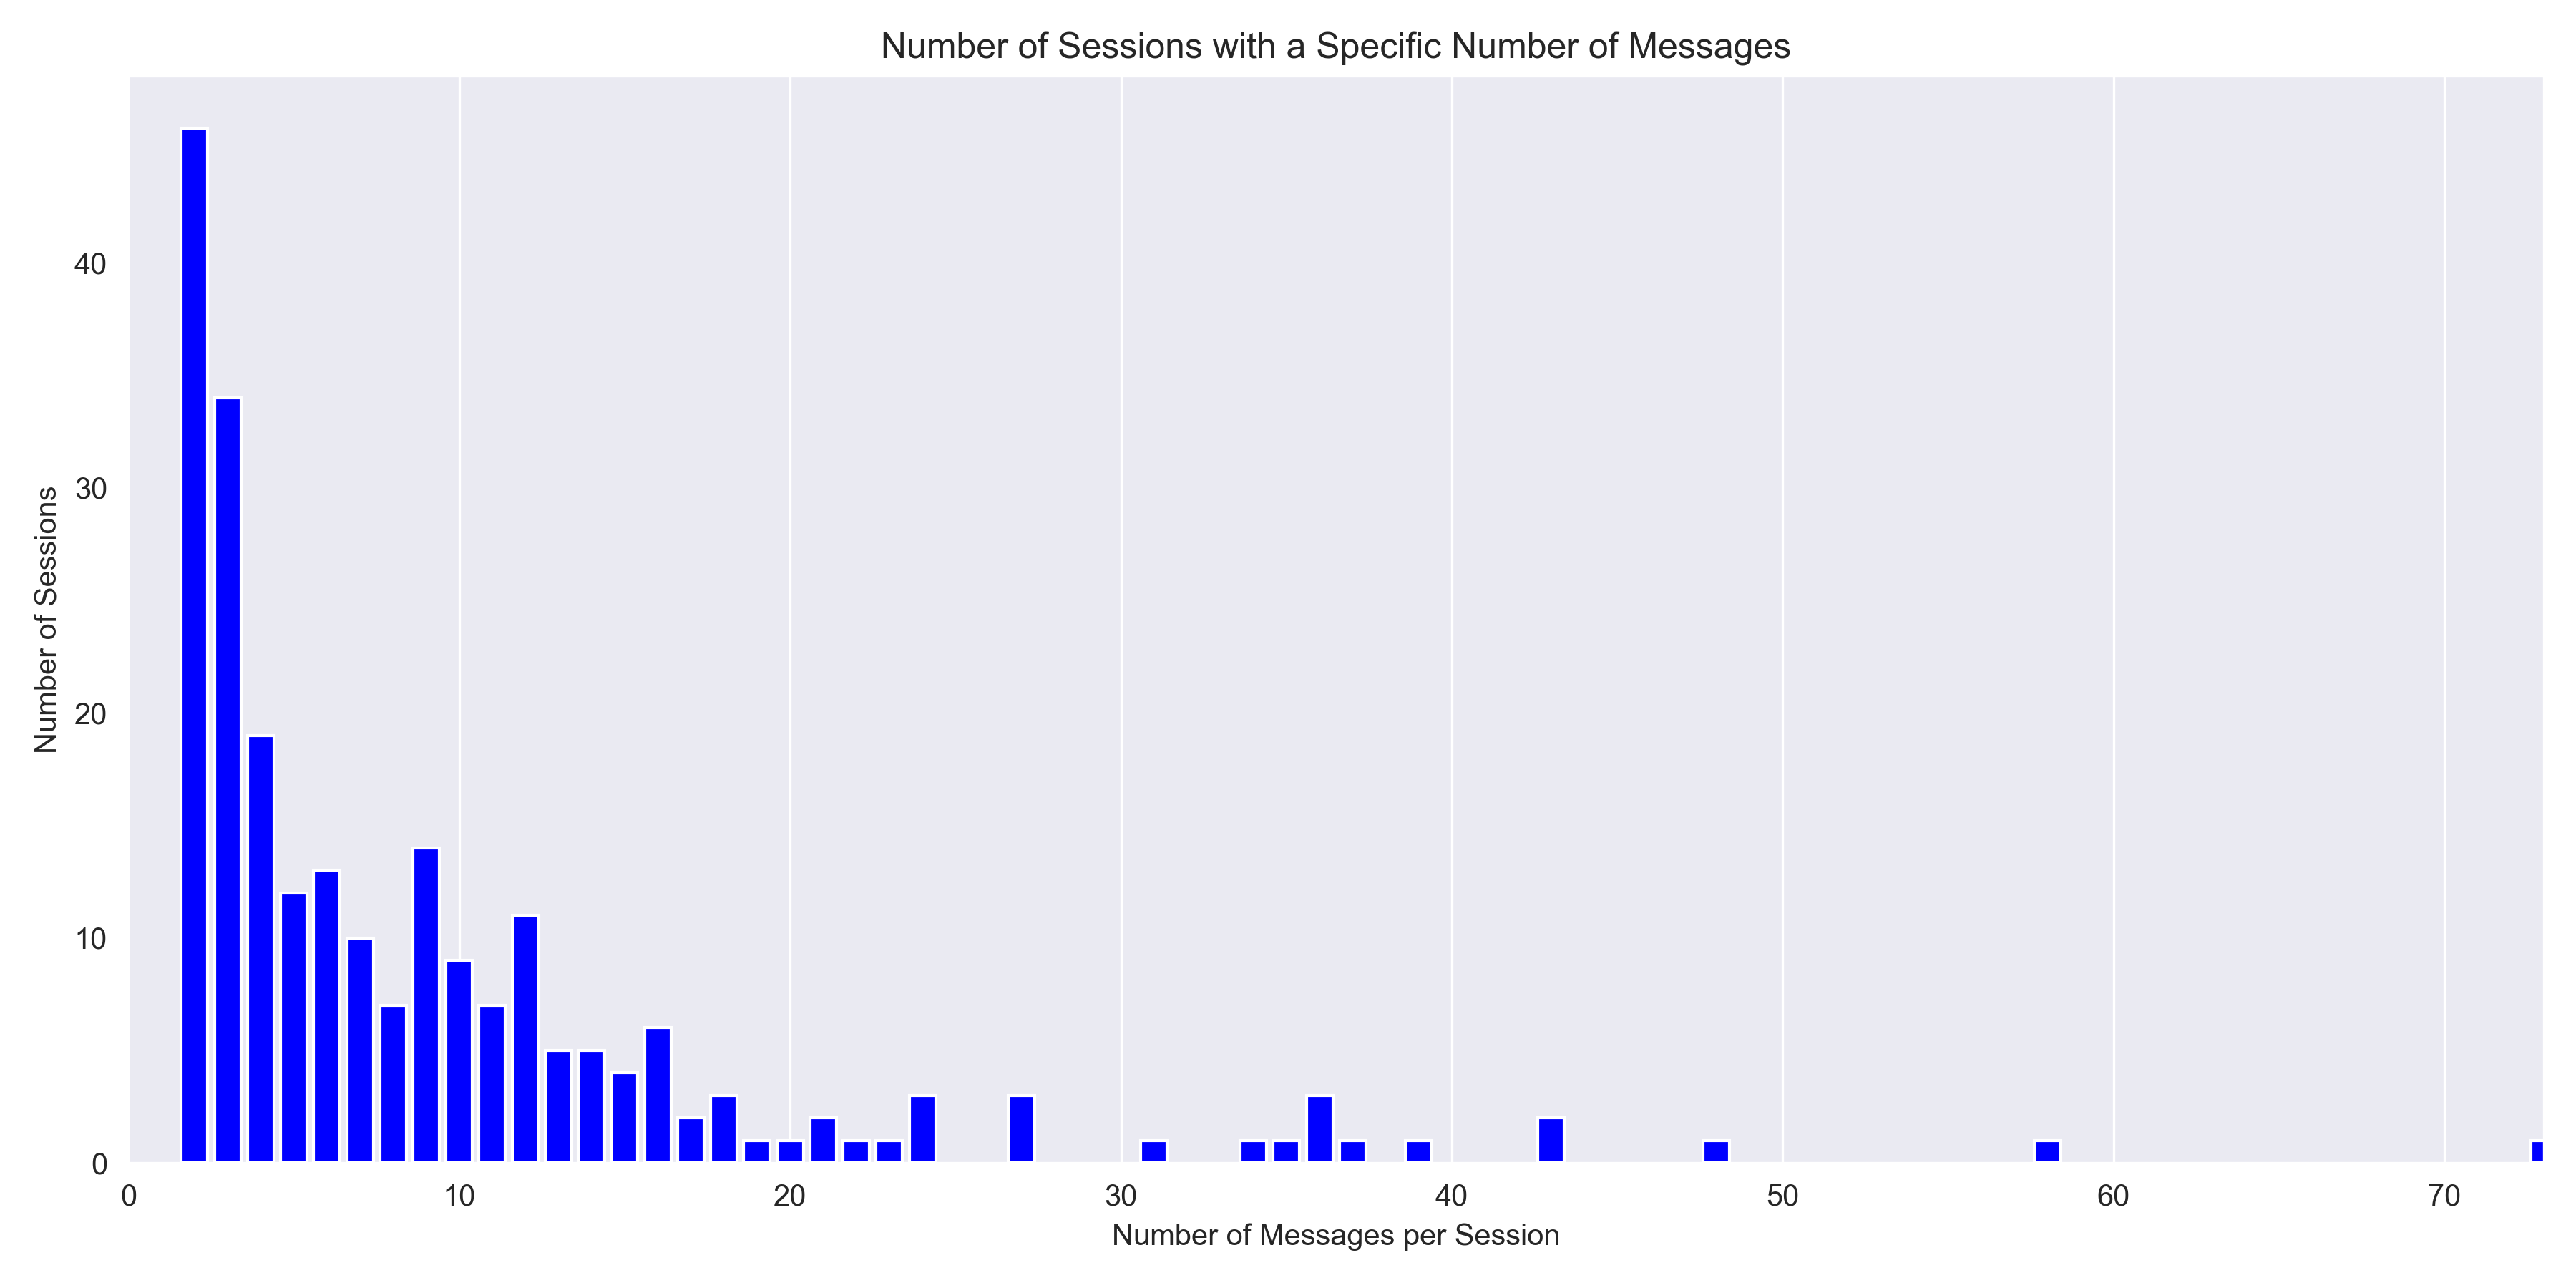
\includegraphics[width=\textwidth]{results/plots/assets/usage-13-number-of-sessions-with-number-of-messages.png}
    \caption{Number of sessions with each number of messages}
    \label{fig:usage_13_number_of_sessions_with_number_of_messages}
\end{figure}


\subsection{Open source v. Proprietary LLMs}


\subsection{Open source v. Proprietary Embedding functions}


\section{The impact of different LLM models on the speed, accuracy and reliability of responses}


This section will present and analyse the gathered data on user preference and technological efficacy of different tools and technologies such as different \gls{RAG} toolchains and \gls{LLM}, as outlined in section~\ref{sec:goals}.


\section{Qualitative analysis of user responses}


This section will present an analysis of the free text answers users have provided in the forms that have been presented in the participating courses.




% \sweExpl{Lite statistik av fördröjningsmätningarna visas i Tabell~\ref{tab:delayMeasurements}. Förseningen har beräknats från den tidpunkt då begäran GET tas emot fram till svaret skickas.}


\section{Reliability Analysis}


% \sweExpl{Analys av tillförlitlighet\\
% Tillförlitlighet i metod och data}


\section{Validity Analysis}


% \sweExpl{Analys av validitet\\
% Validitet i metod och data}


\cleardoublepage